%@+leo-ver=4-thin
%@+node:paran.20140731220748.2032:@shadow Motivation.tex
%@@color
%@@language latex

\chapter{Private views}

In a project with multiple developers situations may arise where you need to make a change to the structure of the source code. This becomes a problem if you also want to limit the impact other developers.  Maintaining your own private view of the source code could be valuable in these circumstances. One way of doing this is by making version control systems aware of refactoring.  Interference with the structure of the source code in each view could then be kept to a minimum, with only what is necessary merged between views. There is already a significant amount of interest already in making diff tools and version control systems refactor aware. Some example of this are as follows:

\begin{itemize}
  \item MolhadoRef \cite{DannyDig} \cite{Dig2008} attempts to incorporate refactoring in version control systems.
  \item Semantic Merge is a series of stand alone diff tools for different languages. 
\end{itemize}

\section{The problems}
%@<<the problem>>
%@+node:paran.20140731220748.2034:<<the problem>>
There are a couple of challenges when collaborating using versioning control systems. We believe that having private views will help address these issues.  

\begin{description}
\item [Repeated structure changes for other software developers.]
%@<<example>>
%@+node:paran.20140731220748.2035:<<example>>
Imagine a situation where you are working jointly on a project with other people. Since you want to collaborate on different aspects of the same source code you have set up the project in a merge based version control system.  You have checked out your own copy of the code so that you can work on the source code without interfering with any of the changes others are making. It is possible that the code will need to be refactored before any of your changes can be added.  This would be a fair judgement call as Fowler claims that the main time to do refactoring is before making any changes \cite{Fowler1999}. You complete your changes and check your code back into the version control system.  While you are doing this other people have been working on the code.  If you manage to check in your code before anyone else you will not need to merge any of your changes.  Anybody who checks in after you however, could have a merge conflict.  A few of conflicts that they experience could be because the changes you made directly compete with the changes they have made. Potentially more conflicts would occur between the changes they have made and the refactoring that you have completed. This is because a refactoring often makes a large amount of global changes to the source code. 

\begin{figure}[!t]
\begin{center}
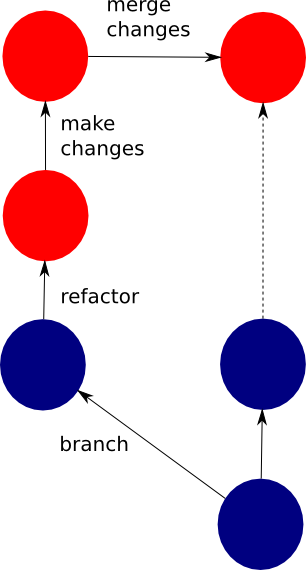
\includegraphics[scale=0.5]{refactorCheckIn}
\end{center}
\caption{Merging changes with refactored code also merges any refactoring}
\label{fig:motMerge}
\end{figure}

As shown in figure Figure ~\ref{fig:motMerge} the difficulty lies in the fact that not only the functionality that you have added is checked in but also the changes brought about by refactoring.  These refactored changes have not changed how the program functions but have simplified and tidied the code to make the addition of your changes easier. These could also include any formatting changes, or code restructuring used to create a programming environment to allow you to be more productive.  During these occasions you may want to avoid changing other peoples code in such a dramatic fashion.

In some conditions refactoring is only required to simplify the code to implement a small change as opposed to cleaning up the entire code base.  This partial refactoring is likely if the code base is large. According to Melina et. al. \cite{Milea2014} refactoring is a challenge when the code base is large. By definition refactoring does not change any functionality, but changes the source code. This means that the code previous to being partially refactored has the equivalent functionality to the code after the partial refactoring.

By checking in your refactoring code you are forcing others to comply with your vision about how the code should be structured.  This occurs even though you could have no awareness about what changes to the code others have made or intend to make.  Everyone who attempts to check in their code after you will need to merge into a restructured code source that they are unfamiliar with.  The potential for merge based bugs and time wasted doing unnecessary merging increases.

%@+at
% then created a branch
% If they attempt to check-in their changes there is the possibility a
% conflict with any of your changes.
% 
% You also need to refactor the code to do your work but both of the
% refactorings are different because they clarify or highlight different
% aspects of the source code.
% 
% If there is some refactoring before any changes are made when the code is
% merged with the original project (often called the trunk project) both
% the changes and the refactored code are checked in.
%@-at
%@@c
%@-node:paran.20140731220748.2035:<<example>>
%@nl
\item [Difficulty if there are multiple check-ins.] 
%@<<multiple checkins>>
%@+node:paran.20140731220748.2036:<<multiple checkins>>
When there is a large change in a separate branch with many development milestones it is desirable to have the ability to submit your code periodically.  This could be done to ensure that there is not too much divergence between the separate branch and other development projects. The desire to regularly merge the code makes the issue we have discussed even worse. Currently if you have a project where there are periodic check-ins for each development milestone there could be a large impact each time there is a commit. This is because any refactoring for the large project is imposed upon others each time it is merged.

%@+at
% One of the ways this can be dealt with is by creating even more branches for 
% different projects however this has some issues with merging when working on 
% two or more projects simultaneously.  In order to minimize the amount of 
% divergence it is advisable to merge each of the branches with the trunk 
% often.  If there has been global refactoring changes introduced by one 
% project being merged the merge will be worse for any of the remaining 
% branches when they are checked in.  Instead of having an issue merging at 
% the check-in level we now have an issue at the merging of branches.  As 
% these changes will occur less often than checking in the code, the code will 
% possibly have more divergence.  This divergence is likely to cause more 
% rather than less merge issues at the expense of having to merge less often.
%@-at
%@@c
%@nonl
%@-node:paran.20140731220748.2036:<<multiple checkins>>
%@nl
\item [Differences in how code is understood.]    
%@<<diff understanding>>
%@+node:paran.20140804074630.2139:<<diff understanding>>
According to  Kerievsky a reason for refactoring code is to better understand it \cite{Kerievsky2004}. As proven by \cite{Bois2005} the very act of going through the source code and reprocessing it in a clearer form can help with the understanding of it. This would suggest that developers tend to leave the code in a difficult to understand state or that different developers understand things differently.
Kerievsky also relates a tale about how the lack of knowledge of patterns makes a particular refactoring look a lot more complex \cite{Kerievsky2004}. The different perspectives meant that the programmer he refers to as John has a differing opinion that the refactored code was not an improvement. This shows that it is not just different functionality that influences the need to refactor but sometime the knowledge and experience of the developers themselves. It is often the case that two developers could have different views about what is an appropriate refactoring. This could be because each person brings different skills, notices different issues and has a preferred way of visualizing a problem and solution.
%@nonl
%@-node:paran.20140804074630.2139:<<diff understanding>>
%@nl
\item [Version control systems not being aware of changes in the order.]
%@<<Change of order>>
%@+node:paran.20140804074630.2144:<<Change of order>>
One of the changes which is not catered for by current version control systems is the changes of order.  The first person to check-in their code will have no issue as the version control system assumes that all the changes are simply a new revision.  When the second person attempts to reconcile their view there is the possibility of having unnecessary conflicts.  A lot of these conflicts will be with refactored code which although works the same has a different structure.
%@nonl
%@-node:paran.20140804074630.2144:<<Change of order>>
%@nl
\end{description}


%@-node:paran.20140731220748.2034:<<the problem>>
%@nl
\section{Benefits of private views}
%@<<benefits>>
%@+node:paran.20140731220748.2038:<<benefits>>
We want to be able to maintain private views that can have different but equivalent refactoring. Different structures of code that function the same way have a number of features that could be of interest.

\begin{description}

\item [Reduced interference with other software developers.]   
%@<<reduced interference>>
%@+node:paran.20140804074630.2140:<<reduced interference>>
One benefit is that it is possible to keep the structure of code that each programmer works on as consistent as possible.  This means that when the developer examines the at the code again that it remains familiar and in a similar state to how it was when they last examined the code. The location of methods and variables are more likely to remain in the place the software developer left them even if a merge occurs.
By maintaining two private views it allows software developers to work on the same programming project to freely refactor or add notes with minimal interference from others.
It also means that the software developer will not interfere with others.
If changes that are purely for formatting are not included when the code is merged then there will be less changes.
The reduced changes would also mean that there will be less merge conflicts when merging code.
%@nonl
%@-node:paran.20140804074630.2140:<<reduced interference>>
%@nl
  
\item [The number of changes is reduced when merging.] 
%@<<reduced changes>>
%@+node:paran.20140805192059.2162:<<reduced changes>>
The number of changes when merging is reduced if you omit any changes that don't also have any change in behaviour.  This in turn means that there is less chance for there to be a merge conflict.
%@nonl
%@-node:paran.20140805192059.2162:<<reduced changes>>
%@nl
  
\item [The ability to have comments tied to a specific view.] 
%@<<personal comments>>
%@+node:paran.20140804074630.2145:<<personal comments>>
It would be possible to have comments that are not considered when doing a merge. This would be a benefit if there are comment that are specific to a view and that are not necessary to share.  This would allow a programmer to keep a lot more personal notes about a change.  As some comments will remain only in private view there is less chance that it will be hard to read the code due to the surplus amount of comments. 
%@nonl
%@-node:paran.20140804074630.2145:<<personal comments>>
%@nl

\end{description}

%@+at
% Can it help with throwaway code or code used for debugging
% 
% When these branches are merged we want to make sure that any source code 
% that is equivalent but refactored is not merged to the view we are merging 
% into. Any source code that changes the behaviour however is considered in 
% the merge.
% 
% We also want to be able to further classify more complex operations in a 
% change set than insert, delete and modify.  When JGit compares files with 
% each other because they are structured it can determine if the file has been 
% moved to a different location in the tree.  At this level JGit can also 
% detect copies and renames.  However once JGit starts comparing source code 
% it loses this structural information.  By giving JGit some idea about the 
% structure in the file it can determine these item at the finer granularity 
% of sections of code rather than at a file basis.
%@-at
%@@c

%@-node:paran.20140731220748.2038:<<benefits>>
%@nl

\section{Implementing private views}
%@<<How achieved>>
%@+node:paran.20140804074630.2143:<<How achieved>>
There are a number of ways we have considered about how to provide private views that have the same functionality.

\begin{description}
  \item [Comparing differences using a non-ordered comparison algorithm.]   
    %@    <<cduanoca>>
    %@+node:paran.20140804193541.2143:<<cduanoca>>
    Instead of using the Longest Common Sub-sequence (LCS) based approach we could instead use a non-ordered comparison.  The easiest way to consider this concept is that the LCS algorithm compares two lists whereas a non-ordered algorithm is a bit more like comparing sets of items. In this illustration each item would be a chunk of code. The items will still need to be ordered.

    %@+at
    % \begin{algorithm}[H]
    % \SetAlgoLined
    % \While{There are elements on both sides that match}{
    % Create a histogram of remaining elements\;
    % Select one of the elements that occurs in both sides the least but not 
    % zero times\;
    % \While{There is an element below the selected one that matches on both 
    % sides}{
    % Remove element from list of elements to compare, as it matches\;
    % }
    % \While{There is an element above the selected one that matches on both 
    % sides}{
    % Remove element from list of elements to compare, as it matches\;
    % }
    % Remove selected element from list of elements to compare, as it 
    % matches\;
    % }
    % \caption{A non-ordered comparison algorithm}
    % \end{algorithm}
    %@-at
    %@@c

    The problems with using this approach to reconcile to different ordered sets is that comparison would not know the difference between what needs to strictly remain in order and what is allowed to be in a different order. If the version control system has an understanding of a particular computer language it is much easier to determine what items can be moved without changing functionality and which ones need to stay in the same order. 
    %@nonl
    %@-node:paran.20140804193541.2143:<<cduanoca>>
    %@nl
  \item [Normalizing the source code before placing it in the version control system.]
    %@    <<Normalising>>
    %@+node:paran.20140804193541.2145:<<Normalising>>
    Before placing the item into source control it could be automatically transformed into an agreed upon format. That is before doing a merge both the code currently in the view and the code that is in source control would need to be transformed into normal form.  Here normal form could mean that all the methods are arranged alphabetically.  Once we have the normal form of both items being merged it will be easier to compare versions to see if they are equivalent.  If both versions are equivalent there is no need to merge them. 

    The number of items that this strategy will resolve however are limited. It also seems more efficient to compare two revisions directly with each other rather than to go to the effort of transforming them before comparing them. 
    %@nonl
    %@-node:paran.20140804193541.2145:<<Normalising>>
    %@nl
  \item [Storing additional information in the version control system.]
    %@    <<Added Info>>
    %@+node:paran.20140804193541.2144:<<Added Info>>
    By storing additional information within the version control system different views could be managed and recreated.
    This concept is very similar to Ekmans plug-in for eclipse that maintains a record different refactorings in addition to the source code \cite{Ekman2004}.

    The problem with this is that it would have to store information about every private view.  In a distributed version control system especially an online one the number of distinct views could be large and change often.   
    %@nonl
    %@-node:paran.20140804193541.2144:<<Added Info>>
    %@nl
  \item [Using regular expressions]
   %@   <<Regular expressions>>
   %@+node:paran.20140807161213.2155:<<Regular expressions>>
   It could be possible to use regular expressions to control a lot of the merge process.  We could eliminate a number of comparisons that contain equivalent functionality in this manner.

   Regular expressions however could be to cumbersome to use to represent a programming language.

    
   %@nonl
   %@-node:paran.20140807161213.2155:<<Regular expressions>>
   %@nl
  \item [Using a tool like JDime solely as a method of comparison.]
    %@    <<Jdime Compare>>
    %@+node:paran.20140804193541.2146:<<Jdime Compare>>
    As mentioned earlier there are a number of reasons why JDime cannot currently be used as a method of keeping two private views. If changed however it could still be useful.  One idea we had was to attach it to Git and solely use it to detect equivalent pieces of java source code.

    The difficulty we experienced with this idea was that JDime had features that we did not want.  Moulding JDime into something that we could use was too complex and it was easier to explore using the JastAddJ compiler. 
    %@nonl
    %@-node:paran.20140804193541.2146:<<Jdime Compare>>
    %@nl
\end{description}

We selected using a non-ordered comparison algorithm as we had a method of figuring out what could be reordered and what had to stay in the same order.  To achieve this we used a parser to discover the AST.  As each AST node had a start and an end position we could relate each AST Node back to its position in the source code.  We could also determine which parts of the source code were comments and white space as these segments of the source code were not covered by an AST node.
%@nonl
%@-node:paran.20140804074630.2143:<<How achieved>>
%@nl

\section{Are comments important?}
%@<<are comments important>>
%@+node:paran.20140807161213.2156:<<are comments important>>
Although in this thesis we have focused mostly on changes to the behaviour of a program as opposed to ascetic changes to the source code we recognise that sometimes changes to comments may be important.  There are occasions were it is practical to require that an important comment or a change to a comment are merged.  There may also be instances where is it better not to merge a comment, as it is specific to this view.  We propose that inserted or deleted comments should be treated as if they are specific to the view and that modifications to existing comments need to be copied into other views.  We believe the best idea however is to allow comments to be marked with an annotation to specify if they are only relevant to the view they are currently in or need to be included in any merge. 

Existing comments and even white space can also provide useful information about any changes of order in the code.  If a programmer has cut and pasted a block of code the white space and comments are also moved and provide hints to what has occurred.  Even if some of the code has been modified there could be enough clues left behind to suggest that the most likely event is that the code has moved and then adjusted.

For these reasons comments are investigated as part of the Refactor Categories tool.

%@+at
% If a new comment is inserted in a branch or even if a comment is deleted it 
% is likely that the change is specific to the task the programmer is trying to 
% implement.  However if an existing comment is modified it is more likely 
% that the comment and the task will have some impact on other branches and 
% should be modified.  There could be exceptions where inserted or deleted 
% code should have an impact on other code and where a modification to a 
% comment does not really need to be broadcast to other users during a merge.
%@-at
%@@c
%@nonl
%@-node:paran.20140807161213.2156:<<are comments important>>
%@nl

%@-node:paran.20140731220748.2032:@shadow Motivation.tex
%@-leo
